\documentclass{llncs}


\usepackage{hyperref}
\usepackage{graphicx}
\usepackage{multirow}
\usepackage[misc,geometry]{ifsym}

\usepackage{amsmath}
\usepackage{enumitem}
%\usepackage{amsfonts}
%\usepackage{amssymb}
%\usepackage{epstopdf}
%\usepackage{epsfig}

\begin{document}

\mainmatter 

\title{Multipoint Approximation Method for Large Scale Design Optimization Problems Under Uncertainty}
\author{Vassili Toropov \inst{1,3} \and Yury Korolev \inst{2} \and Victor Gergel \inst{3} \and Konstantin Barkalov \inst{3} %\Letter 
\\
\email{konstantin.barkalov@itmm.unn.ru}}

\institute{
Queen Mary University of London, London, UK
\and
University of L\"ubeck, Germany
\and
Lobachevsky State University of Nizhni Novgorod, Nizhni Novgorod, Russia
}

\maketitle

\begin{abstract}
The paper presents a new development in the Multipoint Approximation Method (MAM) that makes it capable of handling problems with uncertainty in design variables as well as in additional ‘environmental’ variables. The approach relies on approximations built in the combined space of design variables and environmental variables, and subsequent application of a risk measure and optimization with respect to the deterministic design variables, all within the iterative trust-region-based framework of MAM.

\keywords global optimization, design optimization, multidisciplinary optimization, uncertainty, multipoint approximation method.

\end{abstract}

\section{Introduction}
\label{sec:intro}
In industrial design optimization problems, random inaccuracies of the production process may lead to the designer’s inability to fully control the design variables. Therefore, there can be a discrepancy between the products \textit{as designed} and \textit{as produced} that results in actual performance being different from the performance expected at the design stage. Possible discrepancy between the design and the manufactured product becomes even more important if the latter violates some critical constraints, e.g. safety regulations.

In addition, the system’s performance may depend on parameters of random nature that are beyond the designer’s control, e.g. the operation conditions. Therefore,  accounting for both of these types of uncertainties  is crucial for achieving robust and reliable performance.

Optimization under uncertainty deals with responses $F(\pmb x,\pmb y)$ that depend on deterministic design variables $\pmb x$ and random ‘environmental’ variables $\pmb y$. Uncertainty in the design variables can also be modelled by introducing additional random variables, e.g. as additive or multiplicative noise. In this case, the responses $F(\pmb x,\pmb y)$ receive as input the sum $\pmb x+\pmb u$ (if the noise is additive), where $\pmb u$ is a random variable with a known probability distribution, yielding responses depending on $\pmb x,\; \pmb u$ and $\pmb y$. Randomness in $\pmb u$ and $\pmb y$ induces randomness in the responses $F(\pmb x+\pmb u,\pmb y)$. To convert them into deterministic functions, that can be optimized, a mapping $R$, called the \textit{risk measure} \cite{RockafellarUryasev2000} or \textit{robustness measure} \cite{SchillingsSchulz2015}, is applied to the responses. The result is then a deterministic function of the design variables: $\widetilde{F}(\pmb x)=R(F(\pmb x+\pmb u, \pmb y))$. The choice of a particular risk measure $R$ reflects the designer's attitude towards the risk of sub-optimal performance or constraint violation. For example, $R$ can be a combination of the mean and standard deviation of $F(\pmb x+ \pmb u,\pmb y)$ with respect to the joint probability distribution of $\pmb u$ and $\pmb y$ or a quantile of the distribution of $F(\pmb x+ \pmb u,\pmb y)$, i.e. such a value that the random variable of $F(\pmb x+\pmb u,\pmb y)$ exceeds it with a given, typically small, probability.

Computations of the risk measures typically involve evaluation of high-dimensional integrals, which becomes a challenging task if the number of design variables and/or environmental variables is large. The problem becomes even more difficult if the original responses are computationally expensive, which is the case, for example, in computational fluid dynamics (CFD), where one function evaluation may take hours of even days. Therefore, direct computation of the risk measures using original responses becomes infeasible and therefore approximations of responses, also referred to as metamodels, need to be used.

In problems with a large (in the order of hundreds) number of design variables, the multipoint approximation method (MAM \cite{Toropov1989,Toropov1992,ToropovFilatov1993}) proved to be efficient, e.g. in turbomachinery applications \cite{ShahparPolynkinToropov2008,PolynkinToropovShahpar2008,PolynkinToropovShahpar2010} . This method is an iterative optimization technique based on mid-range approximations built in trust regions. A trust region is a sub-domain of the design space in which a set of design points, produced according to a small-scale design of experiments (DoE), are evaluated. These and a subset of previously evaluated design points are used to build metamodels of the objective and constraint functions that are considered to be valid within a current trust region. The trust region will then translate and change size as optimization progresses. The trust region strategy has gone through several stages of development to account for the presence of numerical noise in the response function values \cite{KeulenToropovMarkine1996,ToropovKeulenMarkine1996} and occasional simulation failures \cite{ToropovMarkineHolden1999}. The mid-range approximations used in the trust regions, as originally suggested in \cite{Toropov1989} for structural optimization problems, are intrinsically linear functions (i.e. nonlinear functions that can be led to a linear form by a simple transformation) for individual sub-structures, and assembly of them for the whole structure. This was enhanced by the use of gradient-assisted metamodels \cite{ToropovFilatov1993}, use of simplified numerical models that is also termed a multi-fidelity approach,\cite{ToropovMarkine1996} and the use of analytical models derived by Genetic Programming \cite{ToropovAlvarez1998}. One of the recent developments \cite{PolynkinToropov2012} involved the use of approximation assemblies, i.e. a two stage approximation building process that is conceptually similar to the original one used in \cite{Toropov1989} but is free from the limitation that lower level approximations are linked to individual substructures.

The Moving Least Squares Method (MLSM) was proposed in \cite{LancasterSalkauskas1981} for smoothing and interpolation of scattered data and later used in the mesh-free form of the FEM \cite{Liszka1984}. As suggested in \cite{ChoiYounYang2001}, it can be used as a technique for metamodelling and used in MDO frameworks. The MLSM is a weighted least squares method where the weights depend on the Euclidean distance from a sample point to where the surrogate model is to be evaluated. The weight value for a certain sample point decays as the distance increases. Describing the weight decay with a Gaussian function tends to be the most useful option even though many others have been evaluated in \cite{ToropovSchrammSahaiJones2005}. As demonstrated in \cite{PolynkinToropov2010}, the cross-validated MLSM can be used both for design variable screening and for surrogate modelling. In order to create an efficient MDO framework for problems with disparate discipline attributes \cite{OllarToropovJones2014} extended the optimization approach of MAM to the use of local DOEs and MLS approximations built in different subspaces of the total design variable space corresponding to the individual disciplines. The subspaces are finally combined into the total design variable space in which the resulting MDO problem is solved.

This paper presents a new development in the Multipoint Approximation Method that makes it capable of handling problems with uncertainty in design variables as well as in additional ``environmental'' variables. The approach relies on approximations built in the combined space of design variables and environmental variables, and subsequent application of a risk measure and optimization with respect to the deterministic design variables, all within the iterative trust-region-based framework of MAM.

\section{The Multipoint Approximation Method}
\label{sec:MAM}

It is useful to start with a brief description of the deterministic version of MAM. A typical formulation of a constrained optimization problem that MAM works with is as follows:
\begin{equation}
  \label{eq:problem}
  \begin{array}{c}
  \min\limits_{a_i \le x_i \le b_i}F_0(\pmb x) \\
  s.t.\; F_j(\pmb x) \le 1,\; j=1,\dots ,M,
  \end{array}
\end{equation}
where $\pmb x$ is the vector of design variables, $\pmb a$ and $\pmb b$ are the lower and upper bounds for the design variables, respectively, $F_0(\pmb x)$ is the objective function, and $F_j(\pmb x)$ are the constraints. The numbers of design variables and constraints are $n$ and $M$, respectively. MAM attempts to solve this problem by using approximations of the objective function and constraints in a series of trust regions. The trust region strategy seeks to zoom in on the region where the constrained minimum is achieved. It aims at finding a trust region that is sufficiently small for the approximations to be of sufficiently good quality to improve the design, and that contains the point of the constrained minimum as its interior point. The main loop of the MAM is organized as follows.

Algorithm 1 (deterministic MAM).
\begin{enumerate}
\item Initialization: choose a starting point $\pmb x^0$ and initial trust region $[\pmb a^0, \pmb b^0]$ such that $\pmb x^0 \in [\pmb a^0, \pmb b^0]$.
\item At the $k$-th iteration the current approximation to the constrained minimum is $\pmb x^k$, the current trust region is $[\pmb a^k, \pmb b^k] \subset [\pmb a^0, \pmb b^0]$.
  \begin{enumerate}[label=(\alph*)]
    \item Design of Experiments (DoE): a set of points $\pmb x_k^i \in [\pmb a^k, \pmb b^k]$ is chosen to be used for approximation building. Responses are evaluated at the DoE points and approximations are built using the obtained values. Currently, the pool of approximation methods available in MAM consists of a metamodel assemblies \cite{PolynkinToropov2012} and the moving least-squares metamodels \cite{LancasterSalkauskas1981,Liszka1984,ChoiYounYang2001,ToropovSchrammSahaiJones2005}. Other metamodel types could be used as well.

    Denote the approximate objective function and constraints by $\widetilde{F}_0(\pmb x)$ and $\widetilde{F}_j(\pmb x)$, respectively.
    \item The original optimization problem (\ref{eq:problem}) is replaced by the following problem:
    \begin{equation}
      \label{eq:problem_approx}
      \begin{array}{c}
      \min\limits_{a_i^k \le x_i ^k\le b_i}\widetilde{F}_0(\pmb x) \\
      s.t.\; \widetilde{F}_j(\pmb x) \le 1,\; j=1,\dots ,M,
      \end{array}
    \end{equation}
    The approximate problem (\ref{eq:problem_approx}) is solved using Sequential Quadratic Programming (SQP) and the solution of this problem determines the center of the next trust region.
    \item The size of the next trust region is determined depending on the quality of approximations at the previous iteration, on the history of the points $\pmb x^k$, and on the size of the current trust region \cite{KeulenToropovMarkine1996}.
    \item The termination criterion is checked (it is a part of the trust region strategy and depends on the position of the point $\pmb x^{k+1}$ in the current trust region, the size of the current trust region and the quality of approximations). If the termination criterion is satisfied, the algorithm proceeds to step 3. Otherwise, it returns to step 2.
  \end{enumerate}
  \item Optimization terminates. The obtained approximation to the solution of the problem (\ref{eq:problem}) is $\pmb x^{k+1}$.
\end{enumerate}

\section{Optimization Under Uncertainty}

The presence of uncertainties in the responses requires certain reformulations in the problem statement (\ref{eq:problem}). Informally, the optimization problem with uncertainty can be written as follows:
\begin{equation}
  \label{eq:problem_unc}
  \begin{array}{c}
  \min\limits_{a_i \le x_i \le b_i}F_0(\pmb x + \pmb u, \pmb y) \\
  s.t.\; F_j(\pmb x + \pmb u, \pmb y) \le 1,\; j=1,\dots ,M,
  \end{array}
\end{equation}
where the random variable $\pmb u$ represents (additive) noise in the design variables and $\pmb y$ is the environmental variable, representing input to the responses that cannot be influenced by the designer. This problem statement is not precise since the random responses $F_0 (\pmb x+\pmb u,\pmb y),\; F_j (\pmb x+\pmb u,\pmb y)$ cannot be directly optimized. Therefore, a risk measure $R$ needs to be applied to the objective and the constraints:
\begin{equation}
  \label{eq:problem_unc_r}
  \begin{array}{c}
  \min\limits_{a_i \le x_i \le b_i}R_{\pmb u,\pmb y}(F_0)(\pmb x) \\
  s.t.\; R_{\pmb u,\pmb y}(F_j)(\pmb x) \le 1,\; j=1,\dots ,M,
  \end{array}
\end{equation}
where the subscript in $R_{\pmb u,\pmb y}$ indicates that the variables $\pmb u$ and $\pmb y$ ‘collapse’ when the risk measure is applied and the result only depends on $\pmb x$. The choices of risk measure will be discussed in Section \ref{sec:risk}. Here the changes in the Algorithm 1 that are necessary to solve the problem (\ref{eq:problem_unc_r}) are discussed.

First, it needs to be decided on whether to build metamodels for the risk measure $R_{\pmb u,\pmb y}(F_j)(\pmb x)$ or for the original responses $F_j (\pmb x+ \pmb u,\pmb y)$. The first option may seem attractive due to the simplicity of its implementation in Algorithm 1 but the deciding argument has to be that of the computational cost associated with the evaluation of either function. On the one hand, one evaluation of the function $R_{\pmb u,\pmb y}(F_j)(\pmb x)$ involves computing one or several integrals of the original response $F_j(\pmb x+ \pmb u,\pmb y)$ over the distribution of $\pmb u$ and $\pmb y$, which requires many evaluations of the original response. On the other hand, the dimensionality of the argument of $R_{\pmb u,\pmb y}(F_j)(\pmb x)$ is less than that of the argument of $F_j(\pmb x+ \pmb u,\pmb y)$, therefore, in principle, fewer function evaluations are needed to approximate the former than the latter. In practice, this may be a matter of a trade-off between the two abovementioned effects that depends on the proportion between the numbers of design variables $n$ and the environmental variables $n_e$ and on the complexity of the integration method and metamodeling method used. If the number if design variables is significantly larger than the number of environmental variables, which is often the case and which is assumed in this paper, building metamodels for the original responses $F_j(\pmb x+ \pmb u,\pmb y)$ is preferred.

This choice requires some changes in the MAM algorithm, since metamodels are now built in a larger space than the one where optimization is performed in. The changes are summarized below.

Algorithm 2 (MAM under uncertainty).
\begin{enumerate}
%  \item Initialization: choose a starting point $\pmb x_0 \in {\Bbb R}^n$. 
  \item Initialization: choose a starting point $\pmb x_0 \in {\pmb R}^n$. 
	Choose an initial trust region $[\pmb a^0,\pmb b^0]$ in the combined space of design variables and environmental variables. 
	Ensure that the initial guess $\pmb x_0$ belongs to the projection of the initial trust region onto the subspace of design variables. The projection of the initial trust region onto the subspace of environmental variables must cover the region where the realizations of the random variable y are likely to be. The coordinates of the trust region corresponding to the environmental variables will not be changed in the course of optimization. Typically, the trust region along the coordinates corresponding to the $i$-th environmental variable is centered at the mean of the $i$-th environmental variable and has the width of six of its standard deviations.
  \item At the $k$-th iteration the current approximation to the constrained minimum is $\pmb x^k$, the current trust region is $[\pmb a^k,\pmb b^k]$.
  \begin{enumerate}[label=(\alph*)]
    \item Design of Experiments (DoE): a set of points $(x_i^k,y_i^k)\in [\pmb a^k,\pmb b^k]$ is chosen that will be used to build approximations. Responses are evaluated at the DoE points and approximations are built using the obtained values.
    Denote the approximate objective function and constraints by $\widetilde{F}_0(\pmb x, \pmb y)$ and $\widetilde{F}_j(\pmb x, \pmb y)$, respectively.
    \item The original optimization problem is replaced by the following problem:
    \begin{equation}
      \label{eq:problem_u_tilde}
      \begin{array}{c}
      \min\limits_{a_i \le x_i \le b_i}R_{\pmb u,\pmb y}(\widetilde{F}_0)(\pmb x) \\
      s.t.\; R_{\pmb u,\pmb y}(\widetilde{F}_j)(\pmb x) \le 1,\; j=1,\dots ,M,
      \end{array}
    \end{equation}
    The risk measures are calculated using the metamodels obtained in the previous step. Integrals that arise during this process are calculated with respect to the joint distribution of $\pmb u$ and $\pmb y$. This distribution is assumed to be fixed.
    The approximate problem (\ref{eq:problem_u_tilde}) is solved using Sequential Quadratic Programming (SQP) and the center of the next trust region $\pmb x^{k+1}$ is determined as the solution of this problem. The optimization runs in a subspace of the space where metamodels are built: metamodels are defined in the combined space of design variables and environmental variables, whilst optimization runs in the subspace of the design variables.
    \item The trust region is updated. The size of the trust region along the dimensions corresponding to the environmental variables is unchanged. The size of the next trust region along the dimensions corresponding to the design variables is determined depending on the quality of approximations at the previous iteration, on the history of the points $\pmb x^k$, and on the size of the current trust region according to the trust region strategy explained in \cite{KeulenToropovMarkine1996}.
    \item The termination criterion is checked. If the termination criterion is satisfied, the algorithm proceeds to step 3. Otherwise, it returns to step 2
  \end{enumerate}
  \item Optimization terminates. The obtained approximation to the optimum is $\pmb x^{k+1}$.
\end{enumerate}

Summarizing, the key changes introduced to account for uncertainties are (i) metamodels built in the combined space of design variables and environmental variables; (ii) optimization performed in a subspace of the space where metamodels are defined; (iii) additive noise in the design variables; (iv) application of risk measures to transform random responses into deterministic functions.

\section{Risk Measures}
\label{sec:risk}

As it has been already said, a risk measure is a mapping that transforms a random response $F(\pmb x+ \pmb u,\pmb y)$  into a deterministic function that can be optimized. Next we provide some examples of risk measures \cite{RockafellarUryasev2000,SchillingsSchulz2015}.

\begin{itemize}
  \item $R(F)=\mu(F)$ where $\mu(F)$ is the mean of $F$. This choice corresponds to optimizing average performance of the system. In typical engineering applications, however, this is not sufficient and more conservative risk measures need to be chosen.
  \item $R(F)=\sup(F)$. This is the most conservative case, in which one is concerned with the worst case performance of the system. The expression $\sup(F)$ stands for the least of all values that are greater than the random response $F$ with probability 1. If the support of the probability density function (PDF) of $F$ is not compact (i.e. $F$ can take arbitrary large values with non-zero probability) than $\sup(F)$ will be infinite.
  \item $R(F)=\mu(F)+k\sigma(F)$, where $\sigma(F)$ is the standard deviation of $F$ and $k>0$ is a constant. This risk measure is sometimes referred to as the safety margin. Optimization using this risk measure is referred to as robust design optimization \cite{KochYangGu2004,Yao2011,ZhangZhuChenArendt2013} and reflects the paradigms of a ‘$3\sigma$-design’, a ‘$6\sigma$-design’, etc.
  \item $R(F)=q_F(\alpha)$, where $q_F(\alpha)$ is the value of the quantile function, or simply the quantile, corresponding to a given probability $\alpha\in (0,1)$. This choice corresponds to the paradigm of reliability-based design optimization  \cite{AouesChateauneuf2010,Yao2011,YounChoi2004}. In this approach, one wants to keep the probability of the system failing (i.e. violating the constraint or underperforming, depending on the context) below a given threshold. The value $1-\alpha$ is the desired probability of failure. Although rather intuitive, this choice has known computational issues which are discussed by Rockafellar and Royset \cite{RockafellarRoyset2010}.
  \item $R(F)=\overline{q}_F(\alpha)$, where $\overline{q}_F(\alpha)$ is the \textit{superquantile} introduced by Rockafellar and Uryasev \cite{RockafellarUryasev2000} and $\alpha \in (0,1)$ is a parameter. The $\alpha$-superquantile can be interpreted as the so-called \textit{buffered probability of failure}. The buffered probability of failure is always slightly more conservative than the usual probability of failure and, therefore, optimizing with respect to the buffered probability, one automatically gets constraints on the conventional probability of failure. It was found by Basova, Rockafellar, and Royset \cite{BasovaRockafellarRoyset} based on a number of engineering examples that the buffered probability of failure typically overestimates the conventional probability of failure by a factor of 3. 	
\end{itemize}

Superquantiles exhibit significantly better numerical properties than usual quantiles \cite{RockafellarRoyset2010}. The $\alpha$-superquantile can also be interpreted either as an average of quantiles  for $\alpha < \beta <1$, or as the conditional expectation of $F$ in its $(1−\alpha)$-tail \cite{RockafellarRoyset2015}:
\[
\overline{q}_F(\alpha) = \frac{1}{1-\alpha} \int_\alpha^1q_F(\beta)d\beta ;
\]
\[
\overline{q}_F(\alpha) = E\left[F|F\geq q_F(\alpha)\right],
\]
where $E\left[F|F\geq q_F(\alpha)\right]$ is the conditional expectation of $F$ (conditional mean). The superquantile corresponding to $\alpha = 0$ is just the mean $\mu(F)=E[F]$.

For this study, we chose two risk measures: the safety margin $R(F)=\mu(F)+k\sigma(F)$ and the superquantile $R(F)=\overline{q}_F(\alpha)$, aiming at covering both robust design optimization and reliability design optimization. Let us briefly discuss its computation.

To compute the safety margin risk measure, one needs to compute two integrals:
\begin{displaymath}
  \begin{array}{c}
    \mu (F)=E[F]=\int F(\pmb x + \pmb u, \pmb y)p df(\pmb u, \pmb y)d\pmb u d\pmb y \\
    \sigma^2(F)=E[(F-E[F])^2]=\\\int(F(\pmb x + \pmb u, \pmb y)-E[F])^2 p df(\pmb u, \pmb y)d\pmb u d\pmb y
  \end{array}
\end{displaymath}

The dimension of these integrals is $n+n_e$. To compute them efficiently, methods of high-dimensional integration must be employed. Here, quasi-Monte-Carlo integration \cite{Caflisch1998} based on Niederreiter sequences \cite{Niederreiter1992} is used.

Computation of the superquantile is not much more involved than calculating expectations, although it is not straightforward to see from its definition. A simple formula for the superquantile exists \cite{RockafellarUryasev2000,RockafellarRoyset2015} that combines computation of an expected value and solution of an auxiliary convex one-dimensional optimization problem:
    \begin{equation} \label{eq:auxiliary_problem}
			\overline{q}_F(\alpha) = \min_c\{c+E[(F-c)_+]\},
    \end{equation}
where where ($F-c)_+$ denotes the positive part of the function $(F(\pmb x+ \pmb u,\pmb y) - c)_+$ (i.e. $F(\pmb x+ \pmb u,\pmb y) - c)$, if this value is positive, and zero otherwise), $E[\cdot]$ is, as before, the expected value, and $c$ is a scalar. It has been shown by Rockafellar and Uryasev \cite{RockafellarUryasev2000} that the function to be minimized in (\ref{eq:auxiliary_problem}) is convex and continuously differentiable in $c$ if the underlying distribution is continuous. Therefore, the minimum in (\ref{eq:auxiliary_problem}) can be easily found using an appropriate one-dimensional convex optimization technique, e.g. the golden search, which was used in the examples in the next section. The integral (expectation) in (\ref{eq:auxiliary_problem}) can be approximated using the quasi-Monte-Carlo method. To solve the auxiliary optimization problem (\ref{eq:auxiliary_problem}), one would need to compute the expectation several times with different values of $c$. It should be noted, however, that this procedure does not require any additional evaluations of the response $F$ as the same samples can be used every time. Therefore, the solution of the auxiliary optimization problem (\ref{eq:auxiliary_problem}) does not present any significant additional computational challenges.

\section{Numerical Example}
\label{sec:num_example}

The example considered in this study is a classical engineering optimization problem known as the scalable cantilevered beam \cite{Vanderpllaats2001}. The engineering object to be optimized is shown in Fig. \ref{fig:beam} taken from \cite{Vanderpllaats2001}.

\begin{figure}[ht]
    \centering
    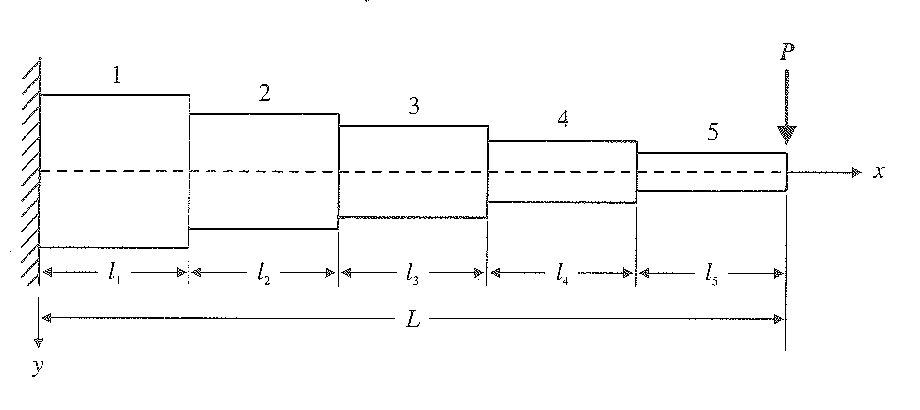
\includegraphics[width=1.0\textwidth]{beam.png}
    \caption{The cantilevered beam}
    \label{fig:beam}
\end{figure}

The design variables are the widths $b_i$ and heights $h_i$ of the segments. The number of segments $N$ can be chosen arbitrary. The total length of the beam is 500 cm, the lengths of the segments are $l_i=500/N$  cm. There are $N$ geometric constraints (the aspect ratios of each block (i.e. heights divided by widths) should not exceed 20) and $N$ constraints on the stress, calculated at the left end of each segment (stresses should not exceed  $\bar{\sigma}=14000\; N/cm^2$). There is also also a constraint on the displacement at the tip, which should not exceed 2.5 cm. The load is $P = 50 000\; N$, the Young's modulus is $E=2\cdot 10^7  N/cm^2$.

The deflection $y_i$ at the right hand of the $i$-th segment is given by the following recursive formulas:
\begin{displaymath}
  \begin{array}{c}
    y_0=y_0'=0, \\
    y_i'=\frac{P\cdot l_i}{E\cdot I_i}\Big[ L+\frac{l_i}{2}-\sum\limits_{j=1}^i l_j\Big]+y_{i-1}', \\
    y_i=\frac{P\cdot l_i^2}{2E\cdot I_i}\Big[L-\sum\limits_{j=1}^i l_j + \frac{2l_i}{3}\Big]+y_{i-1}'l_i+y_{i-1}.
  \end{array}
\end{displaymath}
The moment of inertia of a segment is $I_i=\frac{b_i h_i^3}{12}$ and the bending moment at the left end is $M_i=P[L+l_i- \sum_{j=1}^{i}  l_j ]$. The maximum bending stress in the segment $i$ is then given by the following formula:
\begin{displaymath}
  \sigma_i=\frac{M_i h_i}{2I_i}
\end{displaymath}

We are looking for a design with smallest volume $V = \sum_{i=1}^N b_i h_i l_i$. The widths $b_i$ vary from 1.0 to 10.0 cm and the heights $h_i$ from 5.0 to 100.0 cm. The optimization problem is formulated as follows:
\begin{displaymath}
  \begin{array}{c}
    \min\limits_{\pmb b, \pmb h}V(\pmb b, \pmb h) \\
    s.t.\;1.0\le b_i \le 10.0, \\
    5.0 \le h_i \le 100.0, \\
    y_N\le 2/5, \\
    \sigma_i \le \bar{\sigma}=14000, \\
    \frac{h_i}{b_i}\le 20.
  \end{array}
\end{displaymath}

With $N=50$ segments (corresponding to 100 design variables) the SQP solution of this problem is $V = 63704.598\; cm^3$. MAM obtained the solution $V = 63935.360\; cm^3$, using 1500 function evaluations (as compared to almost 8000 evaluations used by SQP). The number of points in a trust region used to build approximations was 150. The solution obtained by MAM is very close to the reference solution obtained by SQP, except for the last design variable (the height of the last segment), which indicates that the problem is insensitive to this variable near the optimum, making it hard for the metamodels to capture this dependence. Both SQP and MAM solutions are, however, feasible and differ only slightly in the value of the objective function.

Now let us add uncertainty to the problem, adding Gaussian noise with zero mean and variance 0.1 to each design variable. Using the $\mu(F) + k\sigma(F)$ risk measure, we obtain the following problem statement:
\begin{displaymath}
  \begin{array}{c}
    \min\limits_{\pmb b, \pmb h}\mu(V(\pmb b, \pmb h) + k\sigma V(\pmb b, \pmb h)) \\
    s.t.\;1.0\le b_i \le 10.0, \\
    5.0 \le h_i \le 100.0, \\
    \mu(y_N) + k\sigma(y_N)\le 2.5, \\
    \mu(\sigma_i)+k\sigma(\sigma_i)\le \bar{\sigma}=14000, \\
    \mu(\frac{h_i}{b_i})+k\sigma(\frac{h_i}{b_i})\le 20.
  \end{array}
\end{displaymath}

The notation $\sigma$ was used to denote the variance of a response, but it also stands for the maximum bending stresses $\sigma_i$, resulting in somewhat confusing notation $\sigma(\sigma_i )$. Hopefully, this explanation eliminates the confusion. Optimizing $\mu(F) + k\sigma(F)$ with $k = 3.0$ using SQP on original functions, we obtain the value of the deterministic objective (volume of the structure) at the robust optimum $V = 67598.049\; cm^3$. To compute $\mu(F)$ and $\sigma(F)$ at each iteration, 1000 points were used. Multiplied by the number of evaluations of the robust objective $\mu(F) + k\sigma(F)$ (approximately 8000), we get a rough estimate of $8\cdot 10^6$ of the total number of points that SQP used to find this solution.

Solving the same problem using the new version of MAM suitable for problems with uncertainty, we obtain the value of the deterministic objective (volume of the structure) at the robust optimum $V = 67799.335\; cm^3$. To obtain this result, MAM again used 150 points per trust region to build metamodels, which resulted in a total of 1500 function evaluations, which is orders of magnitude smaller than the number of points required if no metamodels are used.

Finally, let us test the performance of MAM in optimization using the superquantile risk measure. The problem statement now is as follows:
\begin{displaymath}
  \begin{array}{c}
    \min\limits_{\pmb b, \pmb h} \overline{q}_\alpha \left(V(\pmb b, \pmb h)\right) \\
    s.t.\;1.0 \le b_i \le 10.0, \\
    5.0 \le h_i \le 100.0, \\    
		\overline{q}_\alpha \left(y_N\right) \le 2.5, \\
    \overline{q}_\alpha \left(\sigma_i\right) \le \bar{\sigma} = 14000, \\
    \overline{q}_\alpha \left(\frac{h_i}{b_i}\right)\le 20,
  \end{array}
\end{displaymath}
where $\overline{q}_\alpha \left(F\right) $ denotes the $\alpha$-superquantile of a response $F$ (i.e. conditional expectation of $F$ in the upper $\alpha$-tail of its distribution). The value of the deterministic objective at the SQP solution in this problem for $\alpha = 1-10^{-3}$ (this corresponds to a probability of failure of $10^{-3}$) is $V = 68056.999\; cm^3$.

Applying MAM to this problem, the value of the deterministic objective was obtained as $V = 68200.668\; cm^3$. Despite the fact that the superquantile uses information in the tail of the distribution, where local approximations used in MAM are not as reliable, the obtained results are very close to the reference SQP solution. The total number of  points used by MAM (i.e. the number of times the beam was analyzed) in this example is 1649.

The $\mu(F ) + k\sigma(F)$ risk measure uses quantities that are estimated in the middle of the distribution --- the mean and the standard deviation. On the one hand, this has the advantage that samples drawn directly from the distribution of the random variables $\pmb u$ and $\pmb y$ are well suited to approximately compute this risk measure. On the other hand, probabilistic interpretation of the obtained results in this case is only possible under the normality assumption for the distribution of $F$; if the actual distribution of $F$ has heavier tails than the normal one, the actual probability of failure will be higher than the one  the system was designed for.

The superquantile focuses on the tails of the distribution, and is better computed using importance sampling with a distribution with heavier tails (in this example, the Student's $t$-distribution was used). Although the superquantile somewhat overestimates the probability of failure (typically by the factor of 3, as reported by Basova, Rockafellar and Royset \cite{BasovaRockafellarRoyset} based on several of engineering examples), it provides a distribution-independent constraint on the probability of failure of an engineering system being optimized.

\section{Conclusion}
\label{sec:conclusion}

Recent developments in the Multipoint Approximation Method made it capable of solving large scale problems with uncertainty in parameters modelled as additional (``environmental'') random variables and uncertainty in the design variables modelled as additive noise. The approach taken combines metamodels built in the combined space of design variables and environmental variables, application of risk measures that map random responses to deterministic functions, and optimization in a subspace of the space where metamodels are defined, all within the iterative and trust-region-based framework of MAM. Performance is demonstrated on a benchmark example of structural optimization known as the scalable cantilevered beam.

\section*{Acknowledgment}
The authors are grateful for the support provided by the Russian Science Foundation, project No. 16-11-10150.

\bibliography{bibliography}{}
\bibliographystyle{nature}

\end{document}
______________________________________________________________________
